\documentclass[a4paper,11pt]{scrreprt}
    %% Used for changing geometry of the page
    %% Cover page text cannot overlay cover sketching/style 
    %% https://ctan.org/pkg/geometry?lang=en
\usepackage{geometry}
    %% Changes language of some packages protocols
    %% e.g., when captioning images: Figure 1. -> Figura 1.
    %% https://ctan.org/pkg/babel?lang=en
\usepackage[portuguese]{babel}
    %% Used for special fonts
    %% Cannot be compiled with pdflatex
    %% https://ctan.org/pkg/fontspec?lang=en
\usepackage{fontspec}
    %% Arial FONT
    \setmainfont{Arial}
\usepackage{subfiles}
    %% More colors and color options
    %% https://ctan.org/pkg/xcolor?lang=en
    %% https://ctan.org/pkg/colortbl?lang=en
\usepackage{xcolor,colortbl}
    %% More tabular options, like dashed/dotted lines
    %% https://ctan.org/pkg/arydshln?lang=en
\usepackage{arydshln}
    %% List of acronyms
    %% https://ctan.org/pkg/nomencl?lang=en
\usepackage[intoc]{nomencl}
    %% Must be called to init nomencl environment  
    \makenomenclature
    %% More images options/settings
    %% https://ctan.org/pkg/graphicx?lang=en
\usepackage{graphics}
    %% Defining subdirectories to image path enviornment
    %% \graphicspath{{sub1}{sub2}...{subN}}
    \graphicspath{{images}}
    
    %% used to handle cross-referencing commands in LaTeX to produce hypertext links in the document
    %% https://ctan.org/pkg/hyperref?lang=en
\usepackage{hyperref}
    %% math environments
    %% https://ctan.org/pkg/amsmath?lang=en

    %% settings
    \hypersetup{
        colorlinks,
        citecolor=black,
        filecolor=black,
        linkcolor=black,
        urlcolor=black
    }

\usepackage{amsmath}
    %% Defining backgrouns, used to make the cover
    %% https://ctan.org/pkg/background?lang=en
\usepackage[some]{background}
    %% Used to make drawings or complex graphics
    %% http://pgf.sourceforge.net/pgf_CVS.pdf
\usepackage{tikz}
    %% Tikz library to point operations ((x1,y1) + (x2,y2))
    \usetikzlibrary{calc}
\usepackage{lscape}
%% Defining sfdefault font and default font for document
\renewcommand{\familydefault}{\sfdefault}


%% Costume made cover 
%% From there you can use \makecover command to build the cover
%% Blue cover color
\definecolor{titlepagecolor}{RGB}{54,95,145}

%==========================================================================
% COLORED BAR ON THE LEFT SIDE
%==========================================================================

\backgroundsetup{
    scale=1,
    angle=0,
    opacity=1,
    contents={
            \begin{tikzpicture}[remember picture,overlay]
                \path [fill=titlepagecolor]
                (current page.north west) -- ($(current page.north west) + (5,0)$)
                -- ($(current page.south west) + (5,0)$)-- (current page.south west);
                \node[color=white] at ($(current page.south west) + (3,4)$) {\bfseries {\fontsize{50}{60} \textsf{SD}}};
                %\node[color=titlepagecolor] at ($(current page.south west) + (5.8,4)$) {\bfseries {\fontsize{120}{60} \textsf{4}}};
            \end{tikzpicture}
        }
}

%==========================================================================
% TITLE PAGE INFO
%==========================================================================

%% Changes values in this field to show information in the cover and back cover about your team/project


%% TITLE
\title{Sistema de gestão de reservas de voos}

%% AUTHORS
\author{
    \begin{tabular} { c c }
        
\includegraphics[scale=0.2]{author/marco.jpg} & 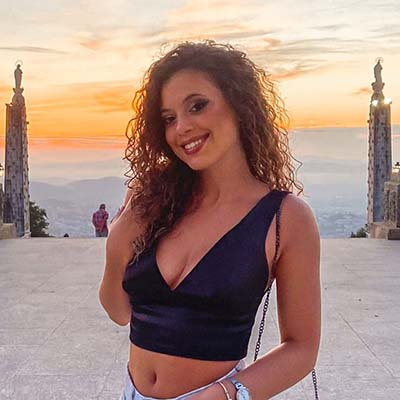
\includegraphics[scale=0.2]{author/mariana.jpg} \\
        62608 - Marco Sousa                           & 93198 - Mariana Marques                       \\
        %\hline                                                                                        \\
        
\includegraphics[scale=0.2]{author/ze.jpg} & 
\includegraphics[scale=0.2]{author/miguel.jpg} \\
        93271 - José Malheiro                         & 94269 - Miguel Fernandes
    \end{tabular}
}

%% Date

\date{\today}

%% Course
\newcommand{\Course}{Licenciatura em Engenharia Informática}

%% Department
\newcommand{\Department}{Escola de Engenharia}

%% UniName
\newcommand{\UniName}{Universidade do Minho}

\newcommand{\UcName}{Sistemas Distribuídos}

\newcommand{\GroupId}{Grupo 12}

%% UniPic
\newcommand{\UniPic}{
\includegraphics[scale=0.09]{uminho.png}}

%% University 
\newcommand{\University}{
    \begin{flushleft}
        \UniPic
    \end{flushleft}
    \textcolor{gray}{\small\textbf{\textsf{\UniName}}}\par
    \textcolor{gray!80!white}{\small{\textsf{\Department}}}\par
    \textcolor{gray!70!white}{\small{\textsf{\Course}}}
}

%% UC
\newcommand{\UC}{
    \begin{flushleft}
        \par\textcolor{titlepagecolor}{  \LARGE\textbf{\textsf{Unidade Curricular de \\ \UcName}}}
    \end{flushleft}
}

%% School Year
\newcommand{\SchoolYear}{
    \small{\textsf{Ano Letivo de 2021/2022}}}


%% Define new command to show title, author and date
\makeatletter
\let\Title\@title
\let\Author\@author
\let\Date\@date
\makeatother

%==========================================================================
% CLASSIFICATION SECTION 
%==========================================================================

%% School Year
\newcommand{\ReceptionDate}{}
%% Responsible
\newcommand{\Responsible}{}
%% Evaluation
\newcommand{\Evaluation}{}
%% Observations
\newcommand{\Observations}{}


%% MAKETEMPLATE
\newcommand{\makecover}{

    %==========================================================================
    % BEGIN COVER PAGE 
    %==========================================================================

    %% Removes page number on footer
    \thispagestyle{empty}

    %% No indentation 
    \setlength{\parindent}{0em}

    %% Put Background defined on \backgroundsetup, in this page
    \BgThispage

    %% Changing geometry to prevent overlay with text
    %% At the end of back cover, geometry is default with \restoregeometry
    \newgeometry{top=3.5cm,left=6cm,right=3cm,bottom=2cm}

    %% builds university info defined previously
    \University
    \vspace{1cm}
    %% builds curricular unity info defined previously
    \UC
    %% builds school year info defined previously
    \SchoolYear

    \vspace*{4cm}
    %% bigger space (i think its the default one) between paragraphs 
    \setlength{\parskip}{1em}

    %% builds title info defined previously
    \par\textbf{\textsf{\huge\Title}}
    \par\textbf{\GroupId}
    \vspace{1cm}
    %% builds author(s) info defined previously
    \par\begin{center}
        \Author
    \end{center}

    \vspace{0.5cm}

    %% builds date info defined previously
    \par\Date
    \restoregeometry
    \pagebreak

    %==========================================================================
    % END COVER PAGE 
    %==========================================================================
}


\graphicspath{ {./assets/} }

% TODO
% ABSTRACT - inclui objetivos e descrição MARCO
% abordar motivo de criar passos e material
% considerações finais

\begin{document}

\pagenumbering{gobble}

% builds the cover
\makecover

%==========================================================================
% BEGIN ABSTRACT PAGE
%==========================================================================

%% Abstract name: \Large font size, flushed left and paragraph skip before abstract content
\renewenvironment{abstract}
{\par\noindent\textbf{\Large\abstractname}\par\bigskip}
{}

\begin{flushleft}
    \begin{abstract}
        %=============
        % How to build an abstract
        % https://users.ece.cmu.edu/~koopman/essays/abstract.html
        %=============
        O aumento da procura individual por viagens, dentro ou fora do país, leva à globalização 
        de vários locais outrora desconhecidos ou inabitados por cidadãos de comunidades estrangeiras...
        Deste modo, tendo em consideração os inúmeros sistemas existentes no mercado que permitem 
        a gestão de vários pedidos concorrentemente efetuados, é notável as possíveis dificuldades
        inerentes a estes problemas. 
        É no sentido de testar os conhecimentos agregados de \textbf{Sistemas Distribuídos}, que foi 
        construída uma solução, usando técnicas e conceitos transmitidos pela equipa docente.
        Assim, foi possível desenvolver a nossa aplicação \textbf{Flight Manager}, uma plataforma
        \textit{servidor-cliente} para lidar com os pedidos relativos à reserva de voos por parte de um cliente.
        \par \textbf{Área de Aplicação}: Sistemas Distribuídos
        \par \textbf{Palavras-Chave}: 
    \end{abstract}
\end{flushleft}

\pagebreak

%==========================================================================
% END ABSTRACT PAGE 
%==========================================================================

%==========================================================================
% BEGIN INTRODUCTION
%==========================================================================

%% Starting page numbering here
\pagenumbering{arabic}

\chapter{Introdução}

O presente relatório foi escrito no âmbito da Unidade Curricular de Sistemas Distribuídos (SD), sendo o
seu principal objetivo apresentar a solução desenvolvida para responder às necessidades advindas de uma 
plataforma \textit{servidor-cliente} para reserva de voos.
É concecionado com a diretiva de facilitar a compreensão e entender o planemamento estruturado que levou
à criação do \textbf{Flight Manager}.

%==========================================================================
% END INTRODUCTION
%==========================================================================

\chapter{Breve Descrição do Enunciado Proposto}

\section{Estratégia Utilizada}

\subsection{Middleware}
\subfile{middleware.tex}

\section{Cliente}
\subfile{cliente.tex}

\section{Servidor}
\subfile{servidor.tex}

\section{Funcionalidades Adicionais}

\chapter{Considerações Finais}
\section{Conclusões}

\section{Trabalho Futuro}

%==========================================================================
% BEGIN LISTA DE SIGLAS E ACRÓNIMOS
%==========================================================================

%% Portuguese babel does not translate this environment
\renewcommand{\nomname}{Lista de Siglas e Acrónimos}

%% Text that can be shown before acronyms list
\renewcommand{\nompreamble}{}

%% acronyms
%%\nomenclature[01]{\textbf{}}{}

%% Show acronyms
\printnomenclature

%==========================================================================
% END LISTA DE SIGLAS E ACRÓNIMOS
%==========================================================================

%==========================================================================
% BEGIN ANEXOS
%==========================================================================

\addchap{Anexos}

%==========================================================================
% END ANEXOS
%==========================================================================

\end{document}